
\subsection{Data description}


\subsection{Estimation methodology}

\subsection{Abnormal returns in the market adjusted model}


\subsection{Short term abnormal returns in the Market Model}

To test hypothesis #1 and #2 of whether negative and positive SDG related events impacts firm value on the short term, we set apart negative and positive events and assess the aggregated development in abnormal returns 10 days before and 10 days after an event. Moreover, we isolate the effect of the individual SDGs to test hypothesis #4 of whether events on some sustainability goals are more relevant for investors than other. We apply the Market Model to measure abnormal returns around an event.   



\subsubsection{Negative news}

The average abnormal returns and cumulative average abnormal returns retrieved from the Market Model are illustrated in table \ref{ST_tab}. The development in AAR and CAAR, along with its corresponding standard error bands with a confidence interval of 95\%, is portrayed in figure \ref{fig:ST_neg_news} to support the analysis from a visual perspective. The y-axis depicts the abnormal return and the x-axis before and after an event. The effect of negative events on average stock behavior is presented by the blue line in the graph, and is mostly negative leading up to an event, which indicates a leakage effect. The impact from negative events is approximately zero until $t = -6$ upon which the AAR decreases steadily until $t=0$, where it bottoms at $-0.36\%$. Subsequently, after the negative event at $t=0$ the AAR increases towards neutrality at zero and remains there for the rest of the window. The CAAR stays negative during the full event window and bottoms on $t=2$ after a large decline of approximately $1.2\%$ from  $t=-5$.
Moreover, the AAR is significantly negative between $t=-2$ and $t=0$ at $95\%$. The same goes for the CAAR after $t=-2$ and the remaining window. Generally, negative news seems to be priced in leading up to and including the identified event day, after which they have limited impact. 

\begin{figure} [H]
    \centering
    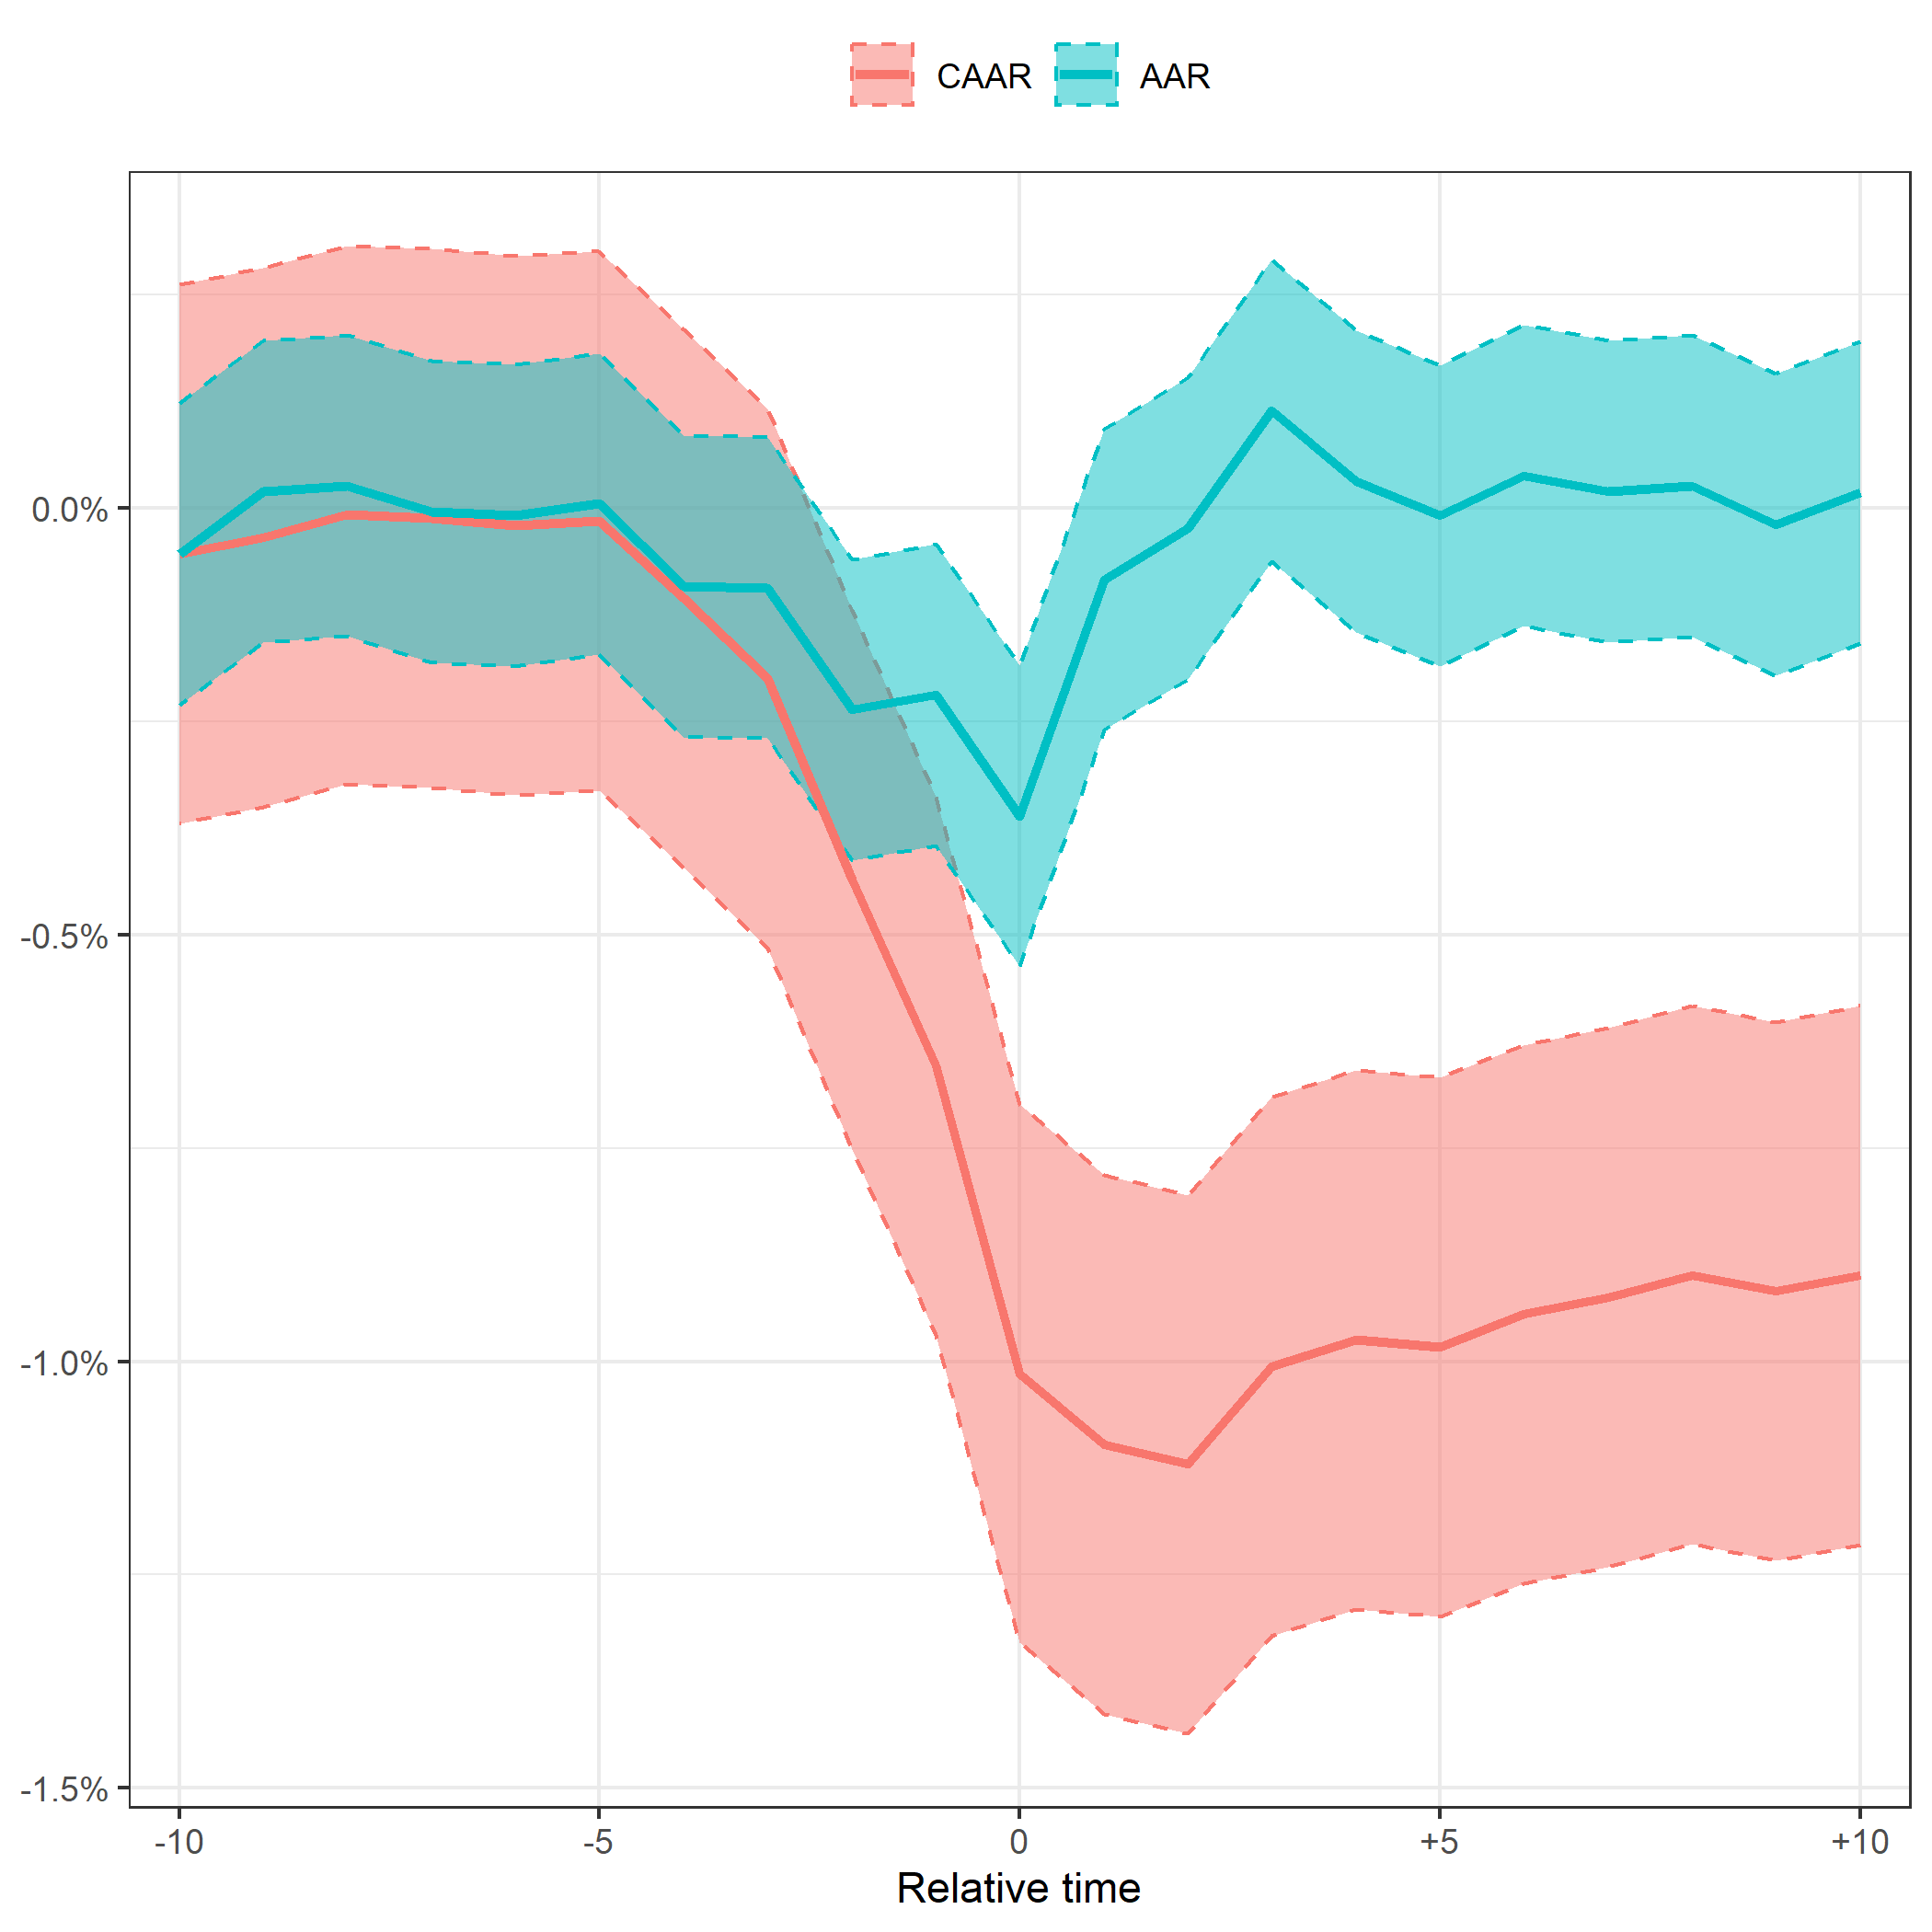
\includegraphics[scale=0.6]{Projekt/1.Figures analysis/ST_negative_all_CI.png}
    \caption{Short term negative news: AAR and CAAR}
    \label{fig:ST_neg_news}
\end{figure}

Examining the average effect from, respectively, positive and negative events provides insights into the overall tendency of the relation between shareholder sentiment and corporate sustainability. By investigating the abnormal returns resulting from events specific to the individual SDGs one can gain a deeper understanding of which themes within corporate sustainability that investors places most emphasis with. Figure \ref{fig:ST_neg_bar} illustrates the aggregated CAAR over the full event window (from $t=-10$ to $t=10$) from events related to specific SDGs along with corresponding confidence intervals.

\begin{figure} [H]
    \centering
    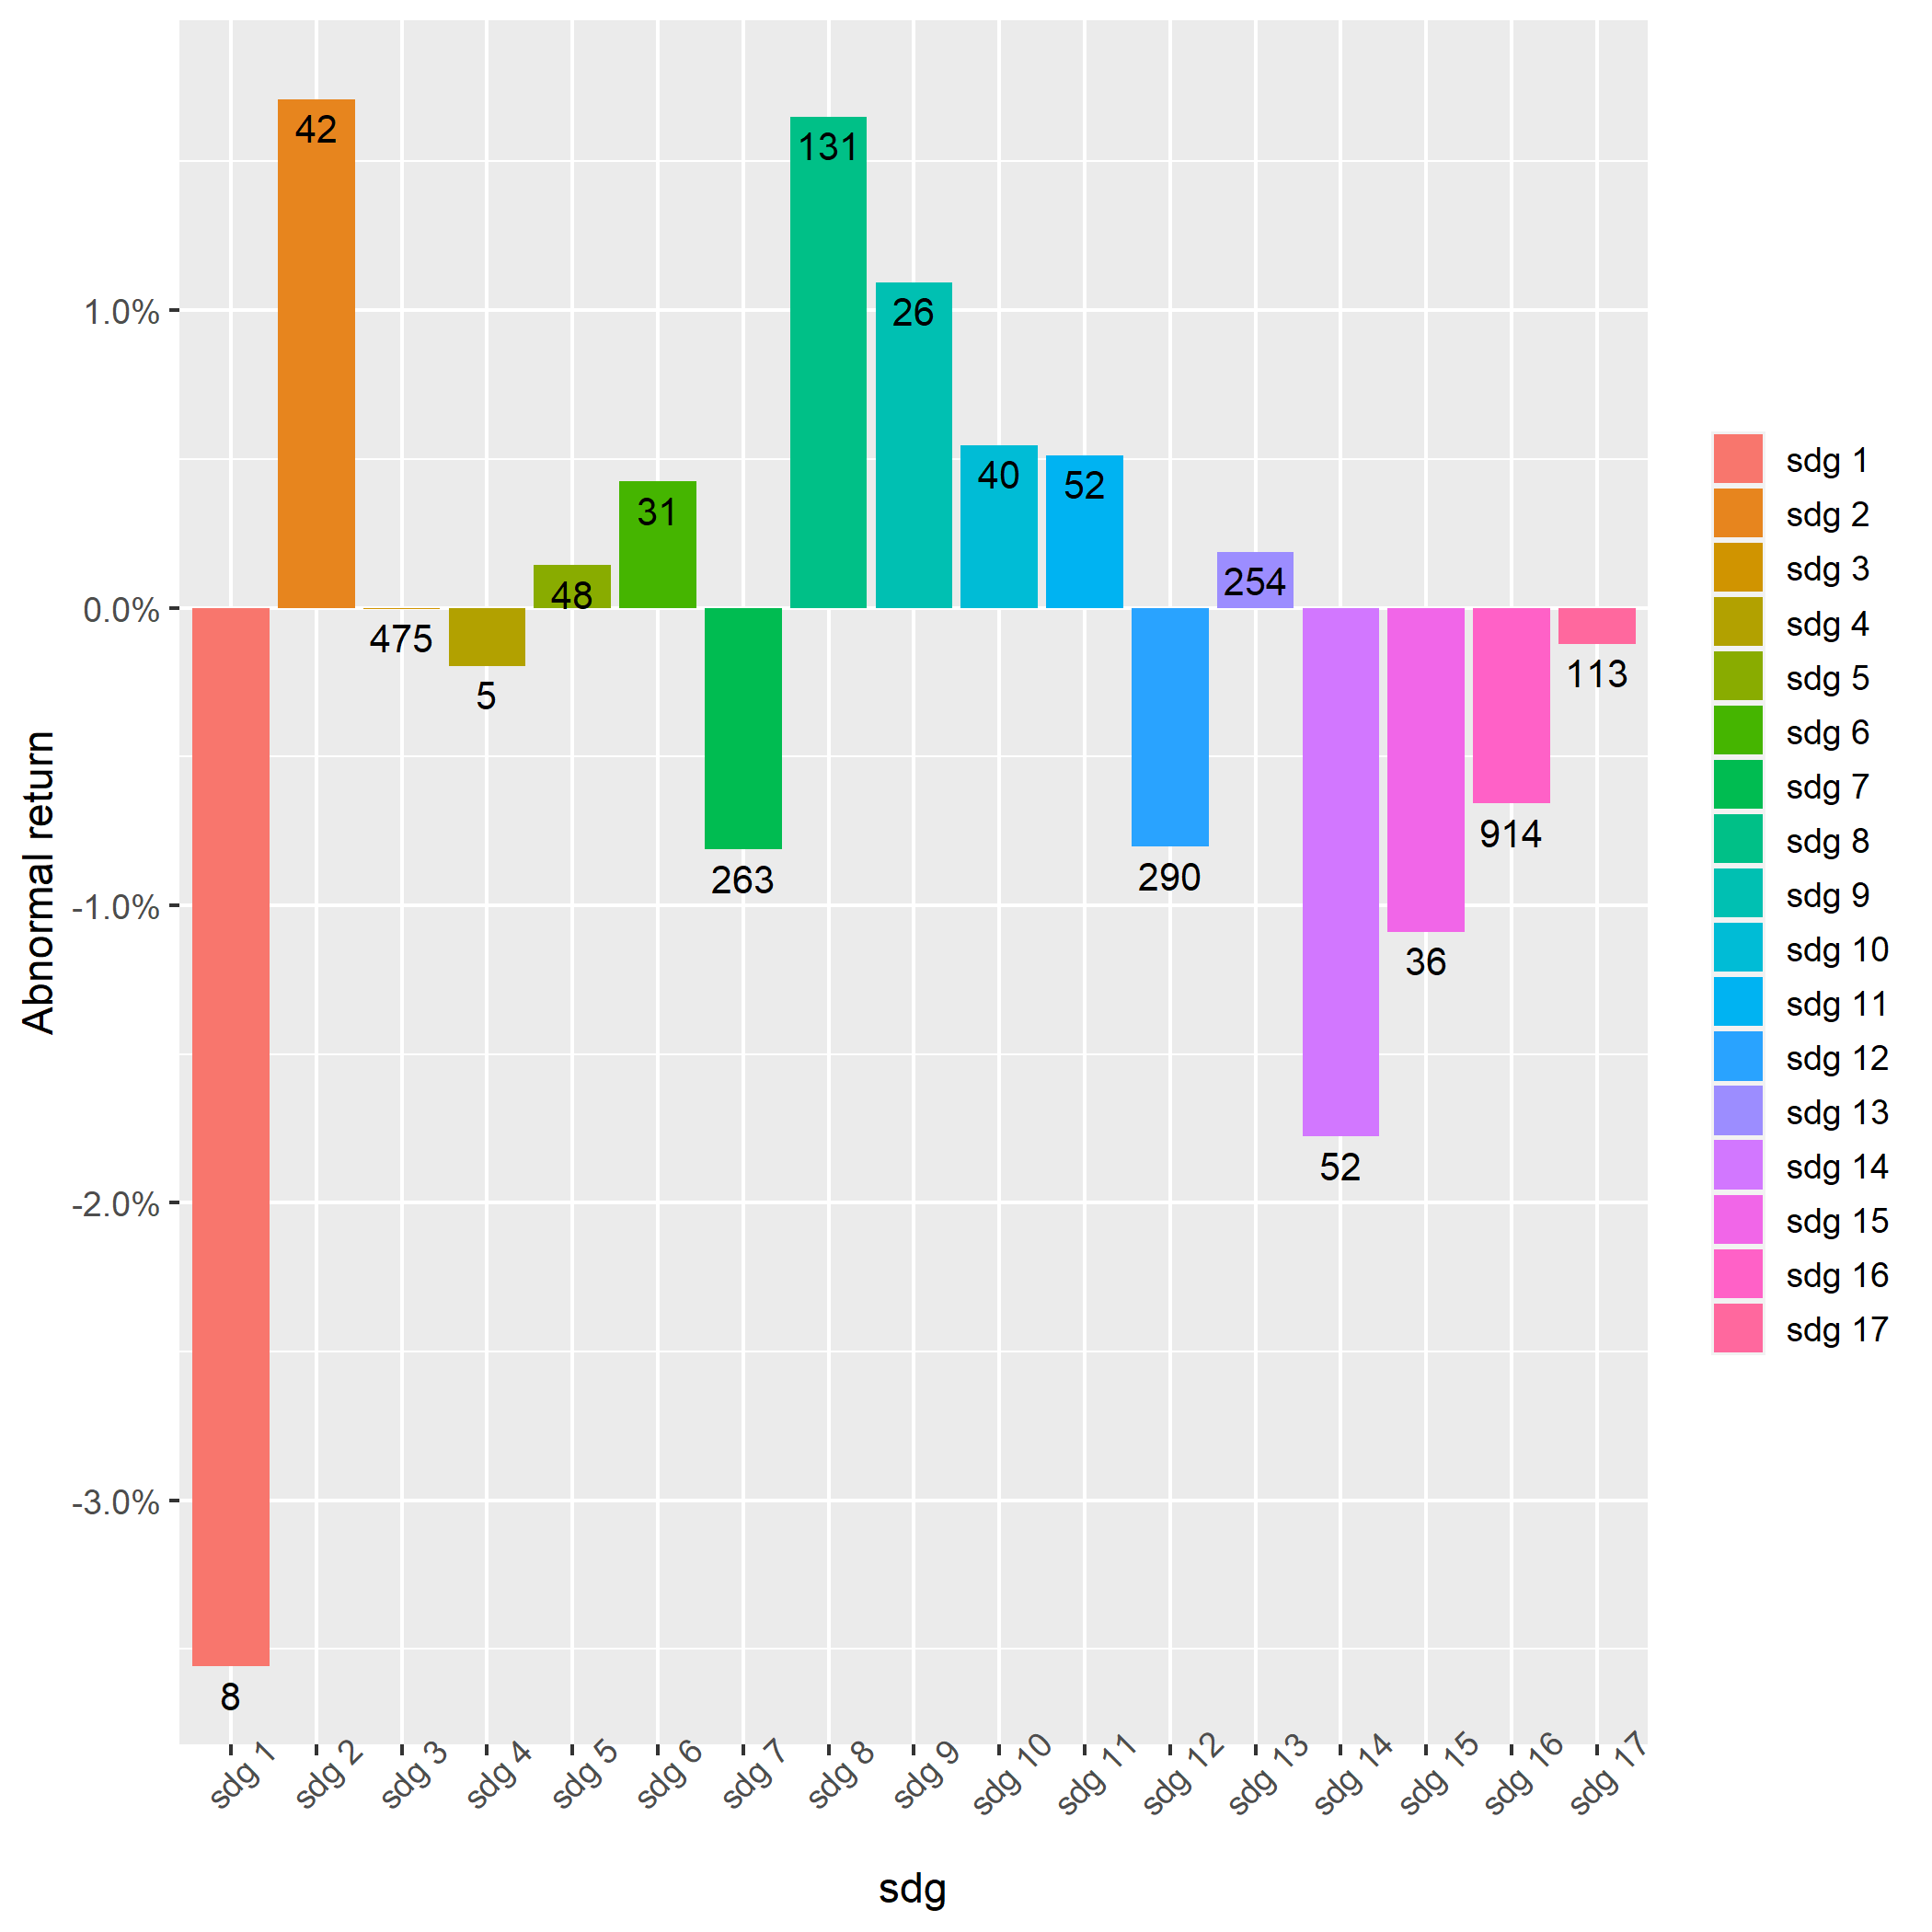
\includegraphics[scale=0.6]{Projekt/1.Figures analysis/ST_negative_sdg_bar.png}
    \caption{CAAR short term negative news}
    \label{fig:ST_neg_bar}
\end{figure}

Splitting the events on SDGs generally illustrate that negative events in most groups are associated with negative abnormal returns. However, the issue of statistical uncertainty in the measurements means that one cannot generate a lot of insights from the aggregated values. Only SDG 15 and 16 alone provides abnormal returns significantly different from zero. The statistical uncertainty originates from the relatively low amount of observations associated with the individual groups after dividing the events into SDGs. For example, SDG 4 has xx observations and a wide confidence interval associated with its mean value, whereas SDG 16 has xx observations and a very narrow band. 


The significance of the results in relation to negative events is summarised with a z-test in table \ref{tab: ST_significace}, which presents the cumulative average abnormal return on $t = 10$ along with the Standard Deviation (SD), Standard Error (SE), Z-score, and the corresponding P-value of the test. The CAAR at $t = 10$ of -.88\% from negative events is significantly different from zero with a Z-score of -1.0914 and a P-value of 0.275. The selection method for negative (positive) events was proposed to round up cases of severe negative (positive) abnormal returns. The result from CAAR clearly shows that abnormal returns are attainable to negative events. However, the method may be late to pick up the signal of negative events or new information on the market. 


\subsubsection{Positive news}

The identified positive events doesn't seem to be associated with any reaction from the shareholders on average, as the AAR doesn't fluctuate significantly from zero at any point during the event window. Following, the statistical uncertainty of the CAAR becomes more widespread through the event window, as indicated by the widening red shadow. However, a slight positive, but insignificant, reaction is visible around the event date. 

\begin{figure} [H] 
    \centering
    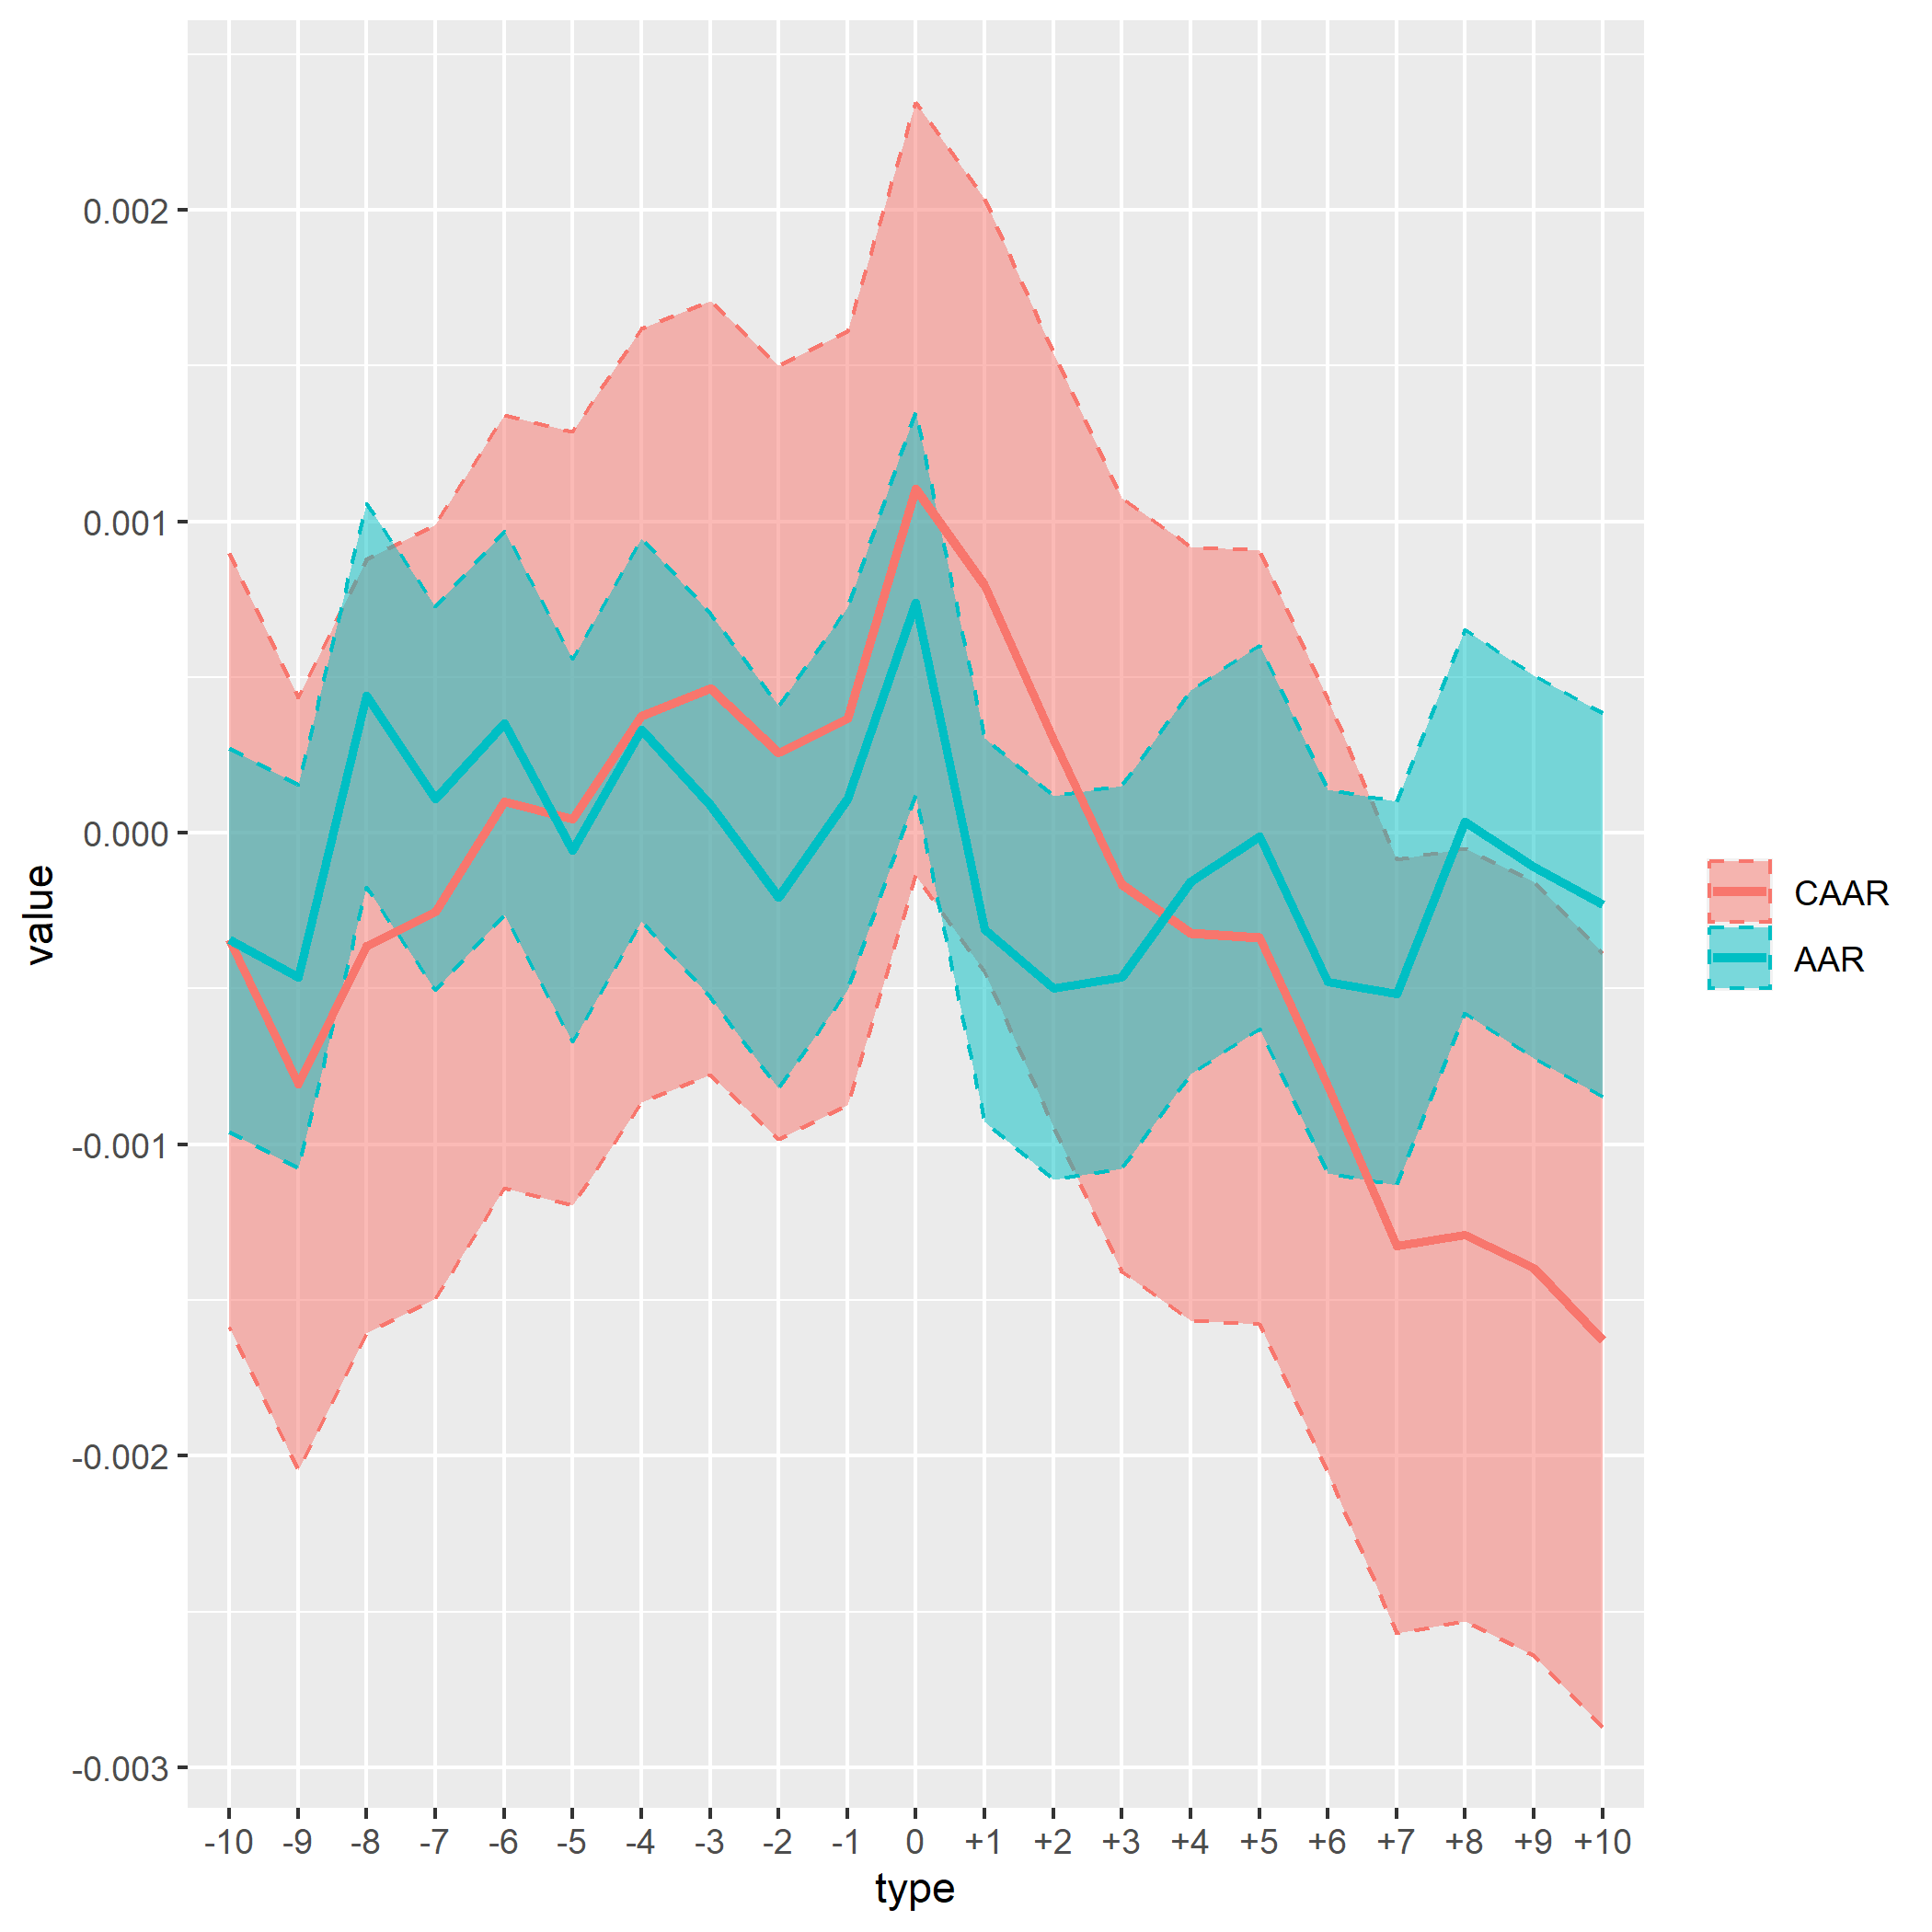
\includegraphics[scale=0.6]{Projekt/1.Figures analysis/ST_positive_all_CI.png}
    \caption{Short term positive news: AAR and CAAR}
    \label{fig:ST_pos_news}
\end{figure}


The tendency of insignificance related to positive events is further reinforced by the results from the individual SDGs, as most are statistically indistinguishable from zero. However, the aggregate do indicate that positive events on SDGs in general are associated with negative abnormal returns. In contrast to the case of negative events, the underlying issue with uncertainty comes with the seemingly random shareholder reaction to positive events.  
 
\begin{figure} [H]
    \centering
    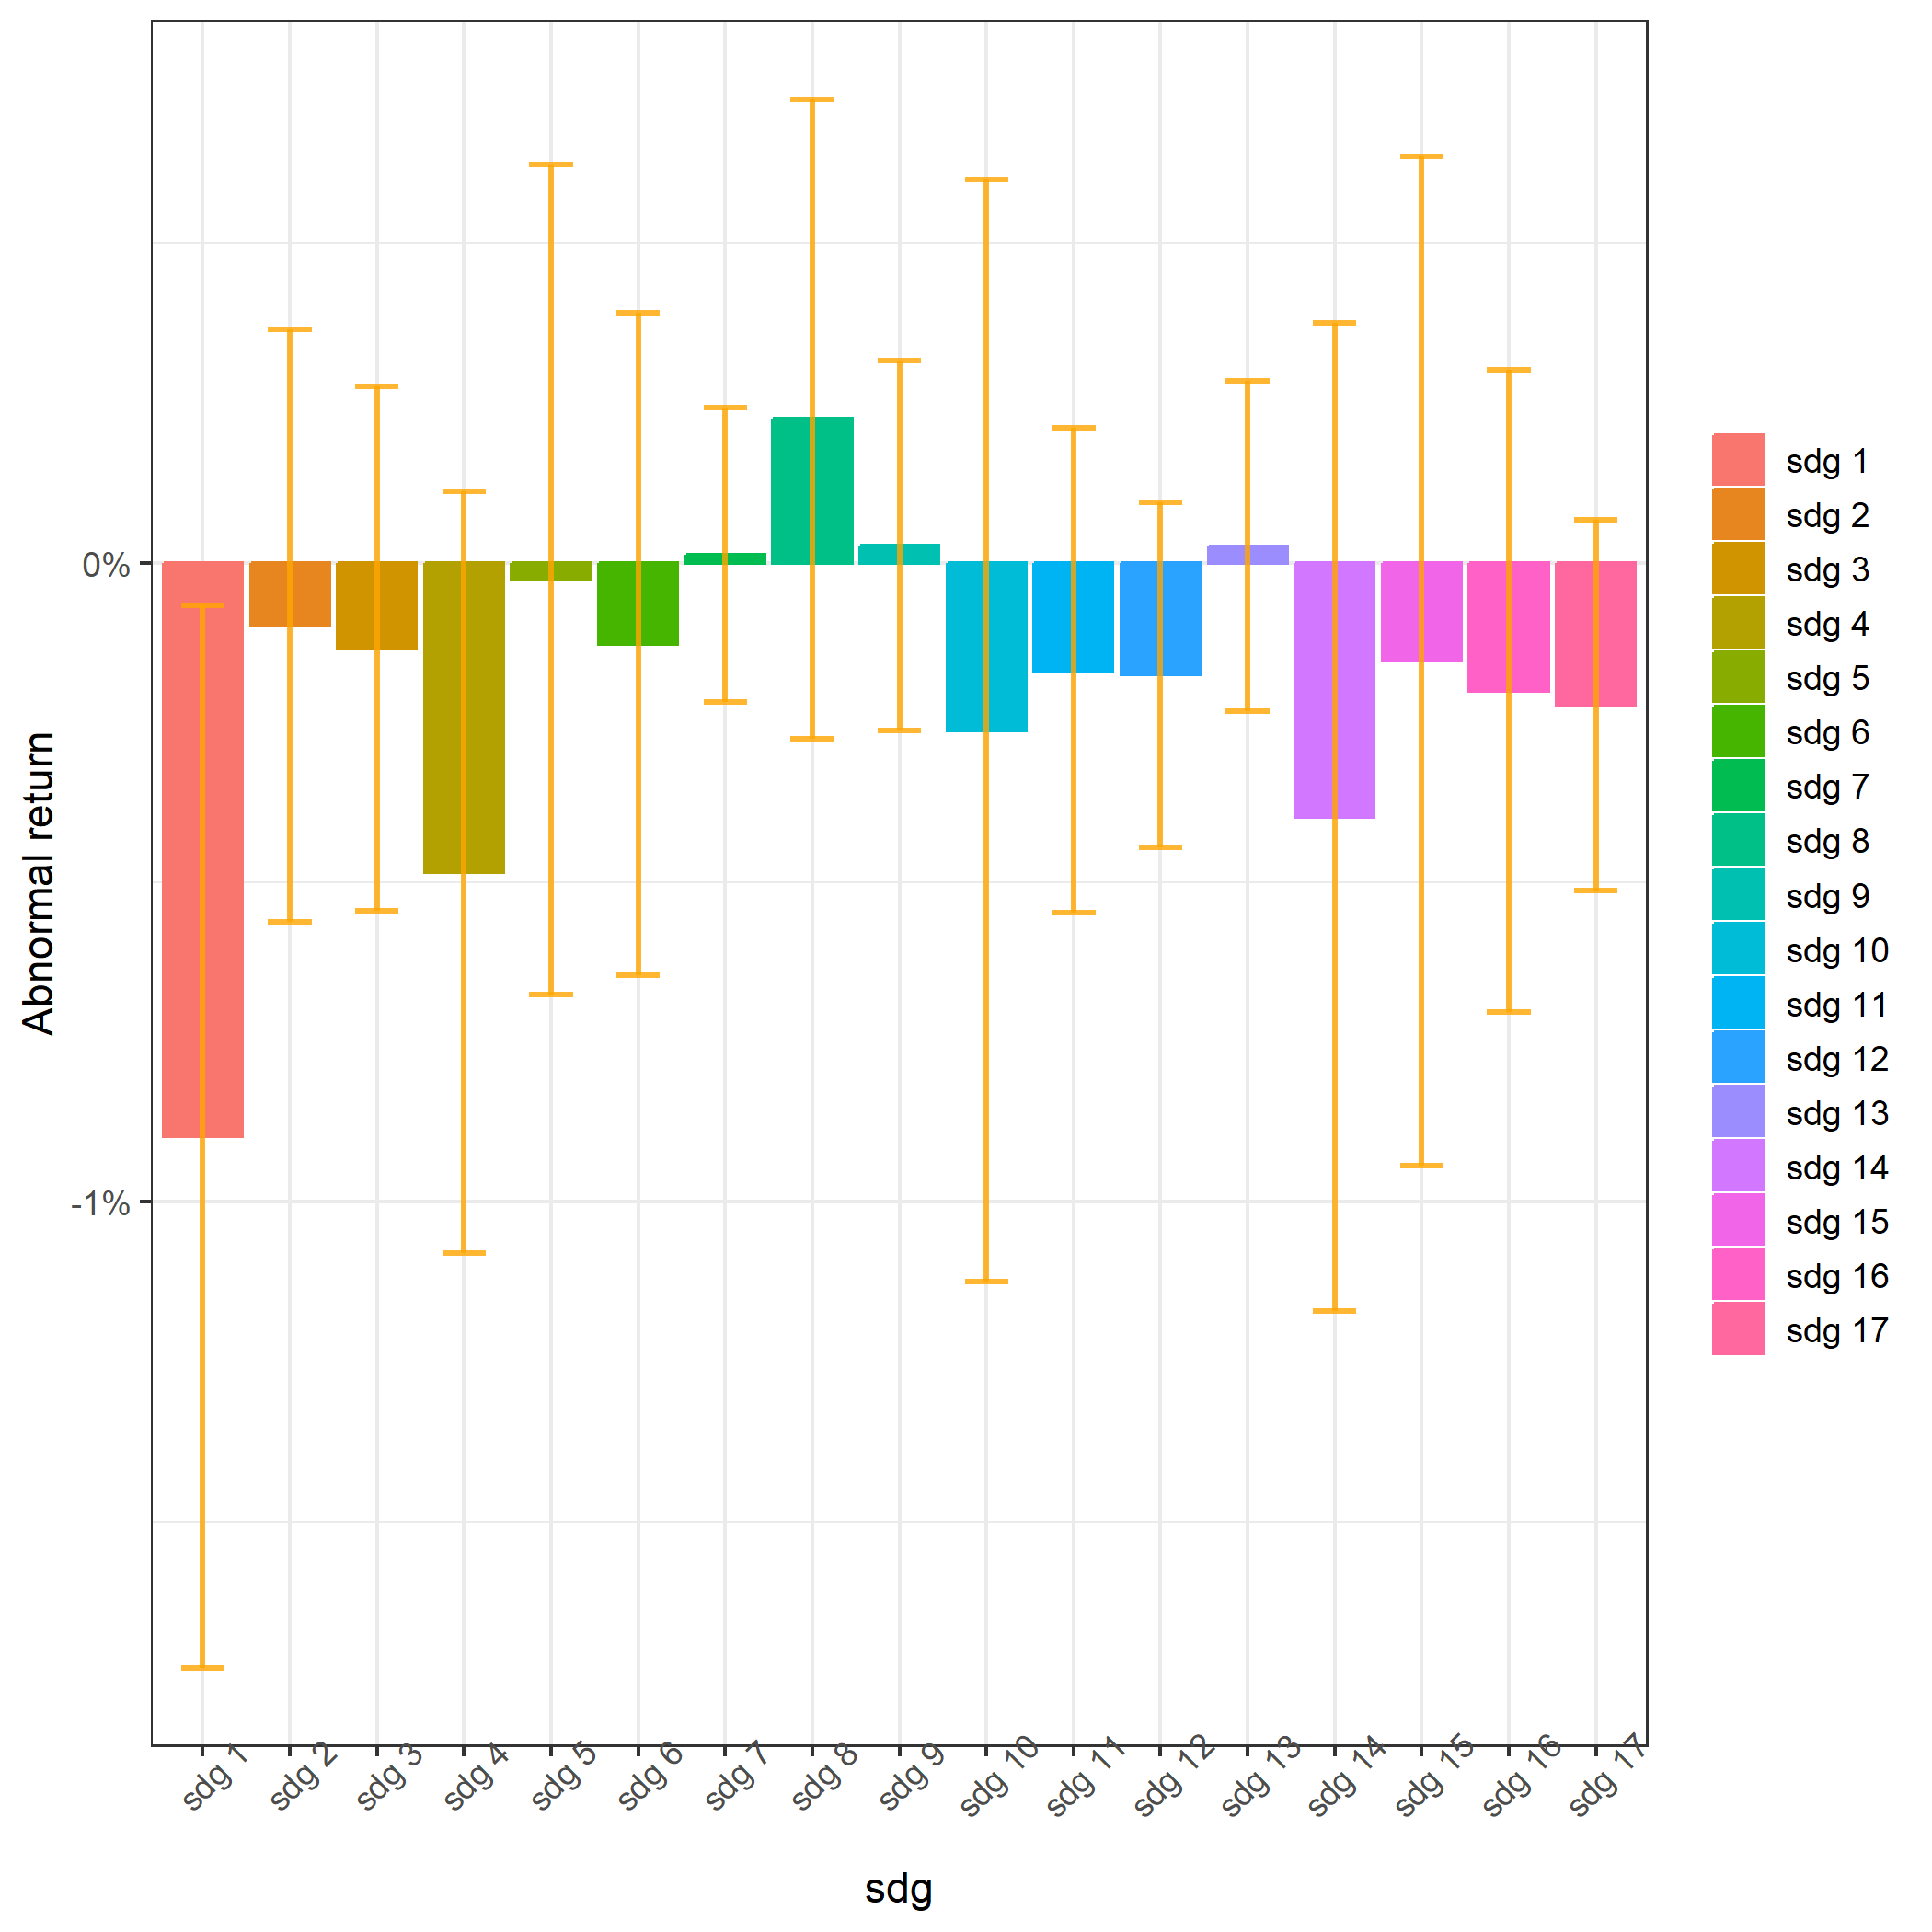
\includegraphics[scale=0.6]{Projekt/1.Figures analysis/ST_positive_sdg_bar.png}
    \caption{$CAAR_{t=10}$: short term positive events}
    \label{fig:ST_pos_bar}
\end{figure}



The insignificance of the abnormal returns associated with positive events are manifested in table \ref{tab: ST_significace}. The z-test of CAAR different from zero has a Z-score of -1.0914 and P-value of 0.27, which indicates insignificance. 

Generally, the short term empirical evidence demonstrate a non-verifiable relation between positive events, related to both broad and specific SDGs, and abnormal returns. The evidence point towards a negative relationship, but this is not statistically valid. 


\begin{table}[ht]
\centering
\begin{tabular}{lllll}
   \hline  \hline
  & $AAR_{t=0}$ & $CAAR_{[-2;+2]}$ & $CAAR_{[-5;+5]}$ & $CAAR_{[-10;+10]}$  \\
 \hline
Positive news & $\underset{(1.973)^{**}}{0.073}$  & $\underset{(-0.211)}{-0.016}$    & $\underset{(-0.379)}{-0.043}$ & $\underset{(-1.091)}{-0.164}$  \\ 
Negative news & $\underset{(-3.457)^{***}}{-0.360}$  & $\underset{(-5.749)^{***}}{-0.917}$    & $\underset{(-4.761)^{***}}{-0.955}$ & $\underset{(-3.288)^{***}}{-0.888}$  \\ 

   \hline
\end{tabular}
\caption{AAR and CAAR over event window (in percentage)} 
\label{tab: ST_significace}
\end{table}



\subsection{Long term abnormal returns}


